\documentclass[
  captions=tableheading,
  bibliography=totoc, 
  titepage=firstiscover,
]{scrartcl}

\usepackage{blindtext} %neuer input

\usepackage{longtable} % Tabellen über mehrere Seiten

\usepackage[utf8]{inputenc} %neuer input

\usepackage{scrhack}

\usepackage[aux]{rerunfilecheck} %Warnung falls nochmal kompiliert werden muss

\usepackage{fontspec} %Fonteinstellungen

\recalctypearea{}

\usepackage[main=ngerman]{babel} %deutsche Spracheinstellung

\usepackage{ragged2e} %neuer input

\usepackage{amsmath, nccmath}

\usepackage{amssymb} %viele mathe Symbole

\usepackage{mathtools} %Erweiterungen für amsmath


\DeclarePairedDelimiter{\abs}{\lvert}{\rvert}
\DeclarePairedDelimiter{\norm}{\lVert}{\rVert}

\DeclarePairedDelimiter{\bra}{\langle}{\rvert}
\DeclarePairedDelimiter{\ket}{\lvert}{\rangle}

\DeclarePairedDelimiterX{\braket}[2]{\langle}{\rangle}{
#1 \delimsize| #2
}

\NewDocumentCommand \dif {m}
{
\mathinner{\symup{d} #1}
}


\usepackage[
  math-style=ISO,
  bold-style=ISO,
  sans-style=italic,
  nabla=upright,
  partial=upright,
  warnings-off={
    mathtools-colon,
    mathtools-overbracket,
  },
]{unicode-math}

\setmathfont{Latin Modern Math}
\setmathfont{XITS Math}[range={scr, bfscr}]
\setmathfont{XITS Math}[range={cal, bfcal}, StylisticSet=1]


\usepackage[
  locale=DE,
  separate-uncertainty=true,
  per-mode=reciprocal,
  output-decimal-marker={,},
]{siunitx}

\usepackage[autostyle]{csquotes} %richtige Anführungszeichen

\usepackage{xfrac}

\usepackage{float}

\floatplacement{figure}{htbp}

\floatplacement{table}{htbp}

\usepackage[ %floats innerhalb einer section halten
  section,   %floats innerhalb er section halten
  below,     %unterhalb der Section aber auf der selben Seite ist ok
]{placeins}

\usepackage[
  labelfont=bf,
  font=small,
  width=0.9\textwidth,
]{caption}

\usepackage{subcaption} %subfigure, subtable, subref

\usepackage{graphicx}

\usepackage{grffile}

\usepackage{booktabs}

\usepackage{microtype} %Verbesserungen am Schriftbild

\usepackage[
backend=biber,
]{biblatex}

\addbibresource{../lit.bib}

\usepackage[ %Hyperlinks im Dokument
  german,
  unicode,
  pdfusetitle,
  pdfcreator={},
  pdfproducer={},
]{hyperref}

\usepackage{bookmark}

\usepackage[shortcuts]{extdash}

%\usepackage{warpcol}


\begin{document}
    \title{ATP Übungsblatt 10}
    \author{  
    Tobias Rücker\\
    \texorpdfstring{\href{mailto:tobias.ruecker@tu-dortmund.de}{tobias.ruecker@tu-dortmund.de}
    \and}{,} 
    Paul Störbrock\\
    \texorpdfstring{\href{mailto:paul.stoerbrock@tu-dortmund.de}{paul.stoerbrock@tu-dortmund.de}}{}
    }
\maketitle
\center{\Large Abgabegruppe: \textbf{Mittw. 10-12 Uhr}}
\thispagestyle{empty}

\newpage
\tableofcontents
\thispagestyle{empty}
\newpage

\setcounter{page}{1}

\section{Aufgabe 28}

\begin{figure}[H]
    \centering
    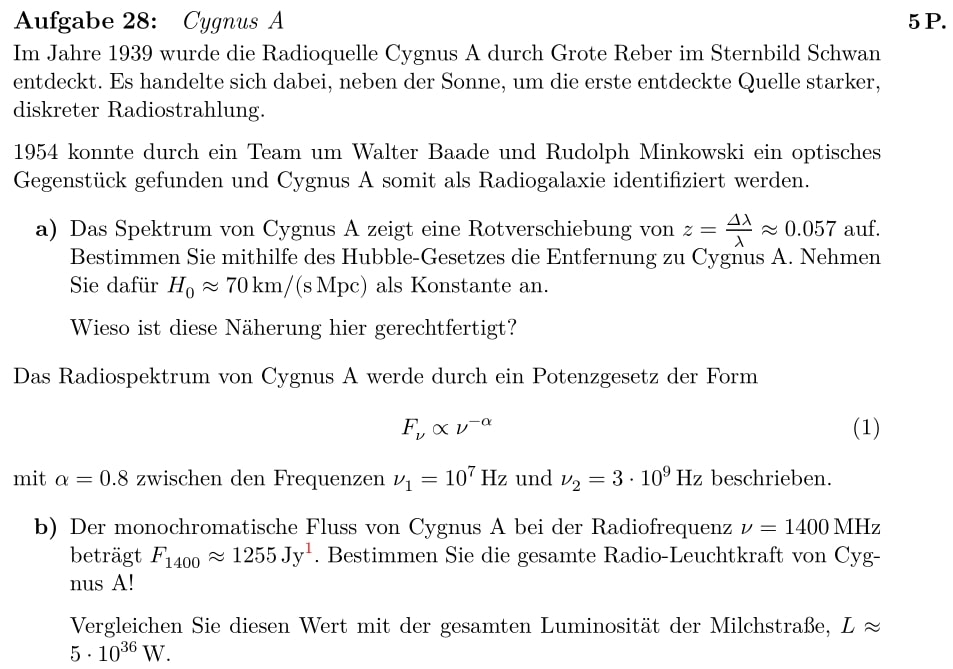
\includegraphics[width=\textwidth]{images/Aufgabe28.jpg}
\end{figure}

\subsection{a)}

    \flushleft{Das\;}\justifying Hubble-Gesetz lautet wie folgt:
    \begin{align*}
        z &= H \cdot \frac{d}{c}
        \intertext{
            \flushleft{wobei\;}\justifying hier die Hubble-Konstante $H$ mit $H_0 \approx 70 \,\text{km s$^{-1}$Mpc$^{-1}$}$ genähert wird.
            $z$ beschreibt die Rotverschiebung und ist hier ungefähr gleich $0.057$, $d$ ist der Abstand und $c$ die Lichtgeschwindigkeit im Vakuum.
            Wird nach $d$ umgeformt, ergibt sich für den Abstand:
        }
        d &= \frac{zc}{H_0} \approx \text{244.117$\,$Mpc}
    \end{align*}
    \flushleft{Die\;}\justifying Näherung der Hubble-Konstante ist hier gerechtfertig, da das Licht <1 milliarden ly an Strecke zurückgelegt hat. Die Hubble-Konstante hat sich
    wahrscheinlich nur im frühen Universum (ca. vor 14 mio Jahren) verändert, da sich das Universum zu der Zeit sehr schnell ausgebreitet hat. Da das Licht nicht aus dem frühen 
    Universum stammt, ist die Näherung der Hubble-Konstante hier gerechtfertigt.

\subsection{b)}

    \flushleft{Das\;}\justifying Radiospektrum von Cygnus A ist durch das Potenzgesetz 
    \begin{align*}
        F_{\nu} &\approx \nu^{-\alpha}
        \intertext{
            \flushleft{gegeben\;}\justifying mit $\alpha = 0.08$ und dem Frequenzintervall $10^7\,\text{Hz} \leq \nu \leq 3\cdot 10^9$. Außerdem beträgt $F_{\nu}\approx 1255\,\text{Jy}$ 
            bei einer Frequenz von $\nu=1400\,\text{\SI{}{\mega\hertz}}$.\\
            Um die gesamte Radio-Leuchtkraft bestimmen zu können, muss die Proportionalitätskonstante des oben genannten Potenzgesetzes bestimmt werden:
        }
        F_{\nu} &= Const\cdot \nu^{-\alpha}\\
        \Leftrightarrow Const &= \frac{F_{\nu}}{\nu^{-\alpha}} = 2.603\cdot 10^{-16}\,\text{\SI{}{\watt\per\hertz\squared\meter\squared}}
        \intertext{
            \flushleft{Um\;}\justifying die Energieflussdichte im Abstand zur Erde bestimmen zu können, muss die spektrale Flussdichte über das Frequenzintervall integriert werden:
        }
        f &= \int_{\nu_1}^{\nu_2} Const \cdot \nu^{-\alpha} \mathrm{d}\nu = Const \int_{\nu_1}^{\nu_2} \nu^{-\alpha} \mathrm{d}\nu\\
        &= Const \left[\frac{1}{\alpha+1} \nu^{-\alpha+1} \right]_{\nu_1}^{\nu_2}\\
        &= \frac{Const}{\alpha+1} \left( \nu_2^{-\alpha+1}-\nu_1^{-\alpha+1} \right)\\
        &= 7.735\cdot 10^{-15}\,\text{\SI{}{\watt\per\meter\squared}}
        \intertext{
            \flushleft{Unter\;}\justifying der Annahme einer isotropen Abstrahlung in alle Richtungen kann die Leuchtkraft $L$ von Cygnus A wie folgt bestimmt werden:
        }
        L &= 4\pi R^2f
        \intertext{
            \flushleft{Der\;}\justifying Radius $R$ ist hier der Abstand zwischen der Galaxie und der Erde $d$. Daraus ergibt sich die Leuchtkraft:
        }
        L_{\text{Cygnus}} &= 5.515 \cdot 10^{36}\,\text{\SI{}{\watt}}
        \intertext{
            \flushleft{Die\;}\justifying Radio-Leuchtkraft der Galaxie Cygnus A ist somit vergleichbar mit der Leuchtkraft der Milchstraße $L\approx 5\cdot 10^{36}$\SI{}{\watt}.
        }
    \end{align*}

\section{Aufgabe 29}

\begin{figure}[H]
    \centering
    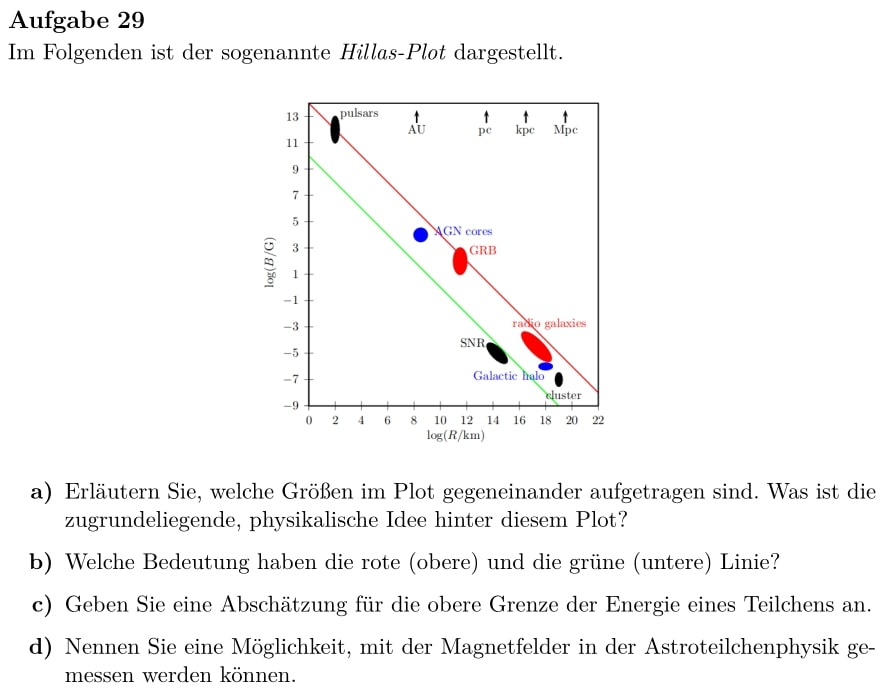
\includegraphics[width=\textwidth]{images/Aufgabe29.jpg}
\end{figure}

\subsection{a)}

    \flushleft{Der\;}\justifying Plot stellt die Größe verschiedener galaktischer Quellen gegen dessen magenetische Feldstärken.\\
    Die physikalische Idee ist, dass verschiedene Arten von Quellen anhand ihrer Größe und relativen Feldstärke den jeweils anderen
    Quellen gegenüber gestellt und verglichen werden können. 

\subsection{b)}

    \flushleft{Die\;}\justifying rote Linie gibt die höchst mögliche Energie (ca. $10^{21}$\SI{}{\electronvolt}) der, von verschiedenen Quellen emittierten, Teilchen an. Die grüne
    Linie gibt die Energie jener Teilchen an, die von dem Magnetfeld der Sonne abgeschirmt werden. Also, die vom termination shock abgelenkt werden und nicht auf der Erde gemessen 
    werden. Alle Energieniveaus zwischen den Linien sind die Energien der Teilchen, die wir auf der Erde messen können. 

\subsection{c)}

    \flushleft{Der\;}\justifying GZK-Cutoff gibt eine mögliche obere Grenze der der Teilchenenergie an. Diese liegt bei ca. $10^{19}$\SI{}{\electronvolt}. Die rote Linie des
    \textit{Hillas-Plot} gibt aber eine obere Grenze von $10^{21}$\SI{}{\electronvolt} wieder. Da der GZK-Cutoff die Wahrscheinlichkeit einer Wechselwirkung des emittierten 
    Teilchens mit den Photonen der CBR. Demnach besteht die Wahrscheinlichkeit, dass es Teilchen mit höheren Energieniveaus gibt, die auf der Erde ankommen. Dies wird durch 
    aktuellen Beobachtungen bestätigt.

\subsection{d)}

    \flushleft{Eine\;}\justifying Möglichkeit ist der Zeemann-Effekt. Dafür wird das Emissionsspektrum eines Sonnenfleckens betrachtet. Im Sonnenfleck selbst wird die Spektrallinie des
    Wasserstoffs in drei geteilt. Dies lässt sich mit den Spinzuständen des Elektrons eines Wasserstoffatoms erklären. Jeder der drei Spinzustände wird unterschiedlich vom Magnetfeld der
    Sonne beinflusst, was sich die Frequenz der jeweiligen Spektrallinie auswirkt. Da dieses Verhältnis zwischen Frequenz und Magnetfeld linear ist, kann daraus die Stärke des Magnetfelds
    bestimmt werden. 

\section{Aufgabe 30}

\begin{figure}[H]
    \centering
    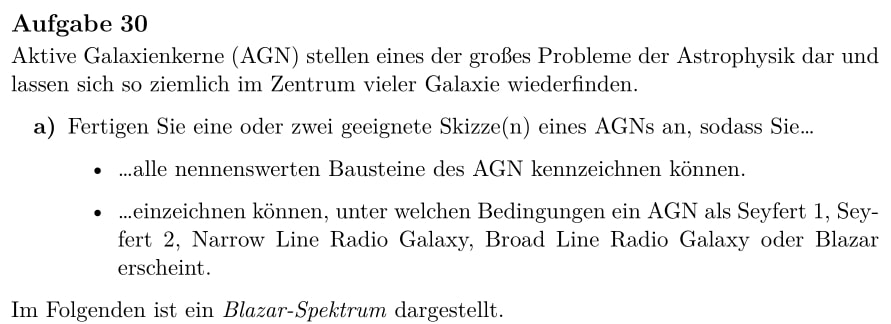
\includegraphics[width=\textwidth]{images/Aufgabe30a.jpg}
\end{figure}

\begin{figure}[H]
    \centering
    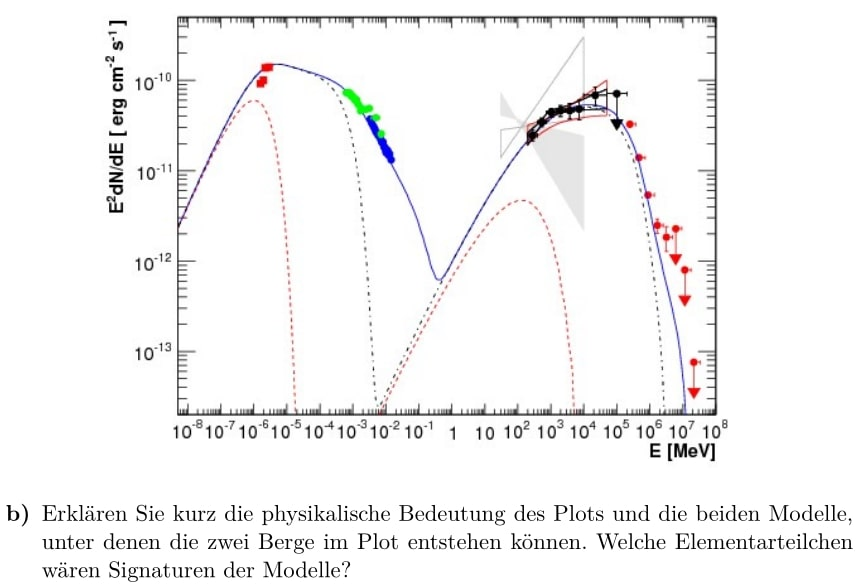
\includegraphics[width=\textwidth]{images/Aufgabe30b.jpg}
\end{figure}

\subsection{a)}

\begin{figure}[H]
    \centering
    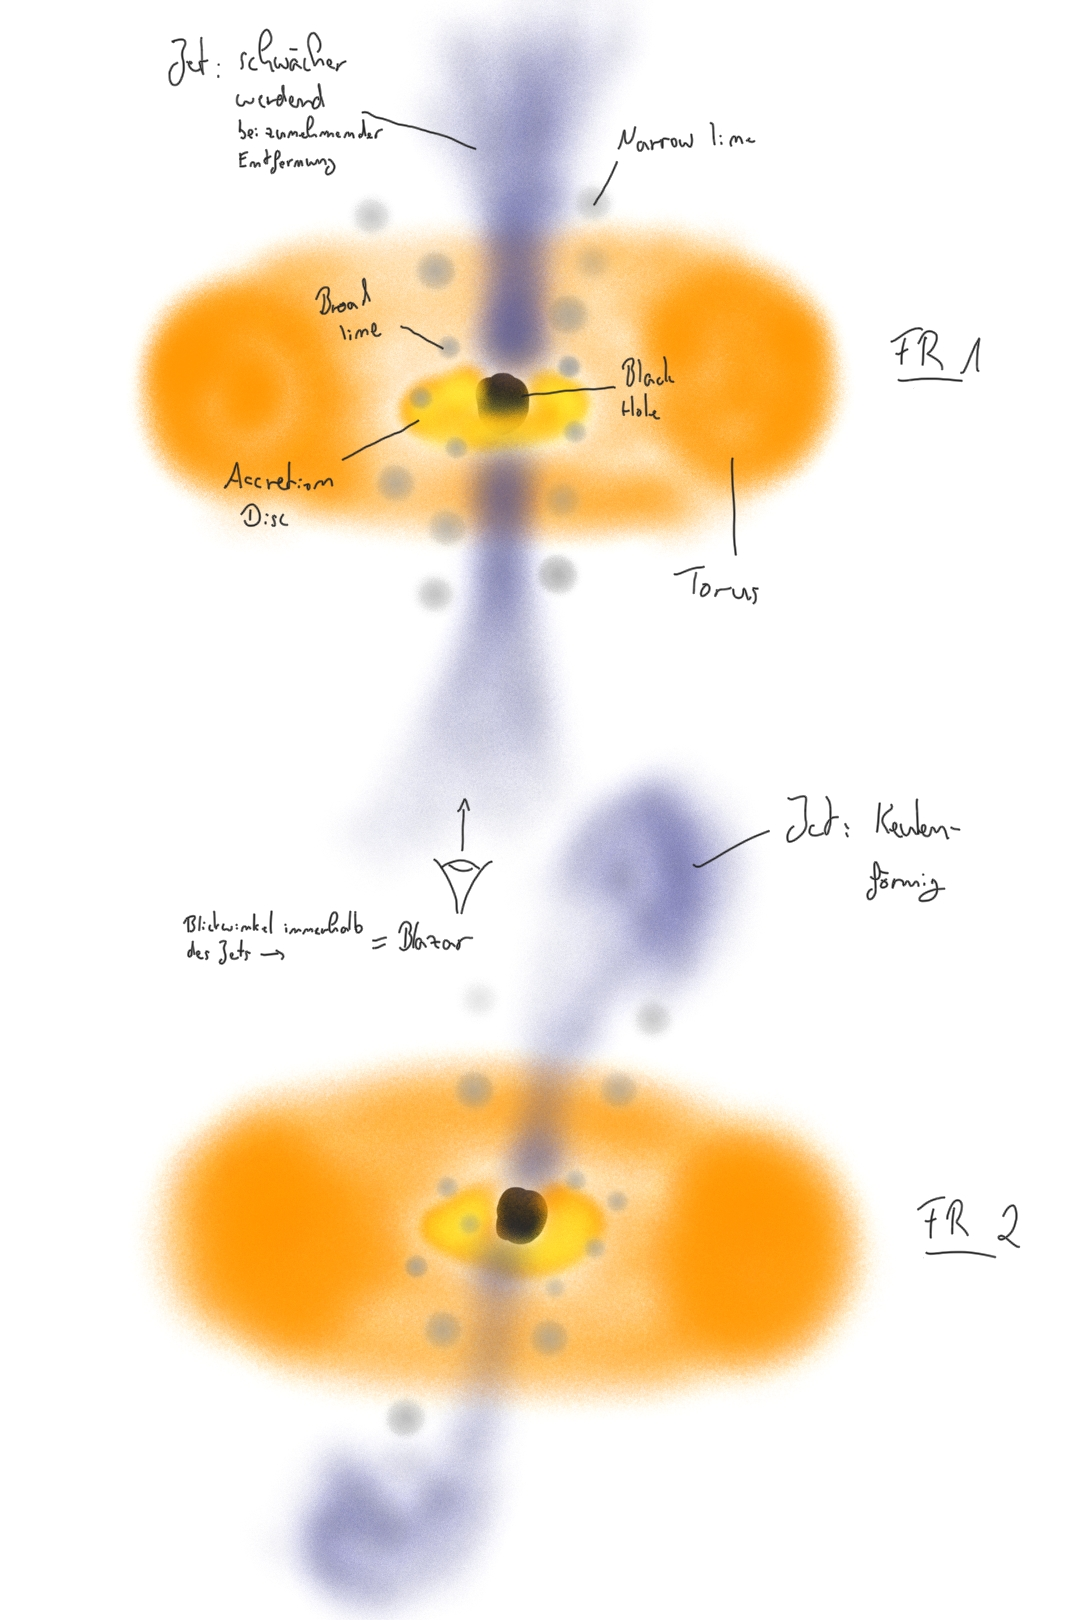
\includegraphics[width=\textwidth]{images/30a.jpg}
\end{figure}

\subsection{b)}
Der Plot stellt das Energiespektrum der Photonen eines AGN's dar, dessen Jet in Richtung der Erde zeigt.
Der jet zeigt dabei zwei charakteristische Höcker, welche auf zwei dominierende Emissionsvorgänge
schließen lässt. Diese ist von nicht-thermischer Strahlung dominiert, kommt von Galaxien mit starken
Radiosignalen und der genaue physikalische Mechanismus dahinter ist experimentell noch unbestätigt.\\
Ein Modell, welches versucht diesen Plot zu beschreiben ist das SSC/EC -Modell: \\
Da wird der 1. Bump durch die Synchrotron-Emission der Elektronen entsteht,
während der Hochenergie-Bump durch inversen Compton Prozess entsteht.
Dabei unterscheiden sich SSC und EC in der Hinsicht, woher die Photonen für
den inversen Compton-prozess kommen. Bei EC Modell wird von externen Photonen von zum 
Beispiel dem Staubtorus oder der Akkretionsscheibe ausgegangen, während beim SSC
Modell die Photonen aus der Synchrotron-Emission mit den Elektronen wechselwirken.\\

Ein anderes Modell bildet das Proton-Blazar-Modell:\\
Hier kommt der erste Bump aus dem gleichen Prozess wie zuvor. Der Hochenergie-Bump 
setzt sich hier aus verschiedenen Beiträgen zusammen. Einer kommt
dabei aus Gammaphotonen aus $\pi ^0$-Zerfällen , welche aus WW von 
Protonen und Photonen kommt.
Ein weiterer Beitrag liefern die Synchrotron-Emission von Protonen und Myonen, wobei
die Myonen aus $\pi ^{+/-}$-Zerfällen stammen.\\

Aus dem $\pi ^+$ -Zerfall entstehen Neutrinos, welche als Botenteilchen für das
Proton-Blazar-Modell gemessen werden könnten.

\end{document}